\documentclass[a4paper, 10pt]{article}
\usepackage[T1]{fontenc}
\usepackage[utf8]{inputenc}
\usepackage[slovene]{babel}
\usepackage{lmodern}
\usepackage{amsmath}
\usepackage{leftidx}
\usepackage{biblatex}
\usepackage{amssymb}
\usepackage{amsthm}
\usepackage{amsfonts}
\usepackage{graphicx}
\usepackage{wrapfig}
\usepackage{amsthm}
\usepackage{mathrsfs}
\usepackage{mathtools}
\usepackage{url}
\usepackage{subfigure}
\usepackage{multirow}
\usepackage{lipsum}
\usepackage{wrapfig}
\usepackage{tikz}
\usepackage[format=plain, font=small, labelfont=bf, textfont=it, justification=centerlast]{caption}
\usepackage{booktabs}
\usepackage{siunitx}

\newtheorem{izr}{Izrek}
\newtheorem{posl}{Posledica}[izr]

\newcounter{defcount}
\newcounter{opombe}
\newcounter{zgledcount}

\newenvironment{opomba}{\begin{flushleft}\stepcounter{opombe}\textbf{Opomba \arabic{opombe}:}}{\hfill\end{flushleft}}
\setlength{\parindent}{0mm}

\newenvironment{zgled}{\begin{flushleft}\stepcounter{zgledcount}\textbf{Zgled \arabic{zgledcount}:}}{\hfill\end{flushleft}}
\setlength{\parindent}{0mm}

\newenvironment{definicija}{\begin{flushleft}\stepcounter{defcount}\textbf{Definicija \arabic{defcount}:}}{\hfill\end{flushleft}}
\setlength{\parindent}{0mm}

\newcommand{\naslov}[1]{\textit{#1}}
\newcommand{\abs}[1]{\ensuremath{\lvert #1 \rvert}}
\newcommand{\mth}[1]{\ensuremath{\mathbb{#1}}}
\newcommand{\R}{\mth{R}}
\newcommand{\Z}{\mth{Z}}
\newcommand{\Zp}{\mth{Z}^{+}}
\newcommand{\N}{\mth{N}}
\newcommand{\No}{\mth{N}_0}
\newcommand{\C}{\mth{C}}
\newcommand{\Qu}{\mth{Q}_u}
\newcommand{\pojem}[1]{\emph{#1}}
\newcommand{\con}{\ensuremath{\mathscr{C}}}
\newcommand{\padex}[2]{\ensuremath{{#1}^{\underline{#2}}}}
\newcommand{\rastx}[2]{\ensuremath{{#1}^{\bar{#2}}}}
\newcommand{\map}[3]{\ensuremath{{#1}: {#2} \rightarrow {#3}}}
\newcommand{\pra}[3]{{#1}{\ast}({#2}) = {#3}}

\title{Projektna naloga pri Statistiki}
\date{17.7.2022}
\author{Jimmy Zakeršnik}
%===============================================================================
\begin{document}
	\maketitle
	\thispagestyle{empty}
	\newpage
	\begin{abstract}
		V tej projektni nalogi pri predmetu Statistika, bom obravnaval tri naloge po navodilih. Vsaka naloga bo obravnavana v svojem lastnem poglavju. Da bo se lažje sklicevati na njih, bo prva naloga poimenovana \pojem{Kibergrad}, druga \pojem{Slučajni sprehod} in tretja \pojem{Temperature}.
	\end{abstract}
	\section{Kibergrad}
	Priložena datoteka \textit{Kibergrad}, ki vsebuje podatke o dani populaciji (prebivalci mesta Kibergrad), je bila odprta v programu LibreOffice Calc. S pomočjo vgrajenega orodja, so nato iz danih podatkov o populaciji bili zbrani vzorci velikosti $500$ po postopku enostavnega vzorčenja. V priloženi datoteki \textit{Kibergradwork} so na prvi strani izpisani vsi podatki ter vseh pet pridobljenih vzorcev, na drugi strani je posebej obravnavan prvi vzorec, na tretji pa medseboj primerjamo vse vzorce glede na dohodek družin tipa $1$. Obe primerjavi izvedemo s pomočjo škatel z brki. Na četrti in hkrati zadnji strani je prikazan izračun variance, pojasnjene s tipom družine, za celotno populacijo, ter izračun rezidualne variance.
	\newpage
	
	\subsection{Primerjava dohodkov med tipi družin prvega vzorca}
	Poglejmo si najprej prvi vzorec in primerjajmo dohodke družin glede na tip družine. Da bo primerjava lažja, jo izvedemo s pomočjo vzporednih škatel z brki. Za vsak tip družine torej poračunamo minimalno vrednost, prvi kvartil, mediano, tretji kvartil in maksimalno vrednost. V prvem vzorcu so te vrednosti naslednje:
	\begin{table}[h!]
		\centering
		\begin{tabular}{|l|c|c|c|}
			\hline
			& Tip $1$ & Tip $2$ & Tip $3$ \\ \hline
			Max & $228727$ & $181696$ & $168926$ \\ \hline
			Q$3$ & $55360$ & $54859$ & $57631$ \\ \hline
			Med & $32975$ & $38883$ & $33310$ \\ \hline
			Q$1$ & $18700$ & $22011$ & $16071$ \\ \hline
			Min & $0$ & $5184$ & $0$ \\ \hline
		\end{tabular}
	\caption{Tabela vrednosti, ki so potrebne za risanje škatel z brki za vsak tip družine}
	\end{table}

S pomočjo zgornjih vrednosti narišemo vzporedne škatle z brki:
\begin{figure}[h!]
	\centering
	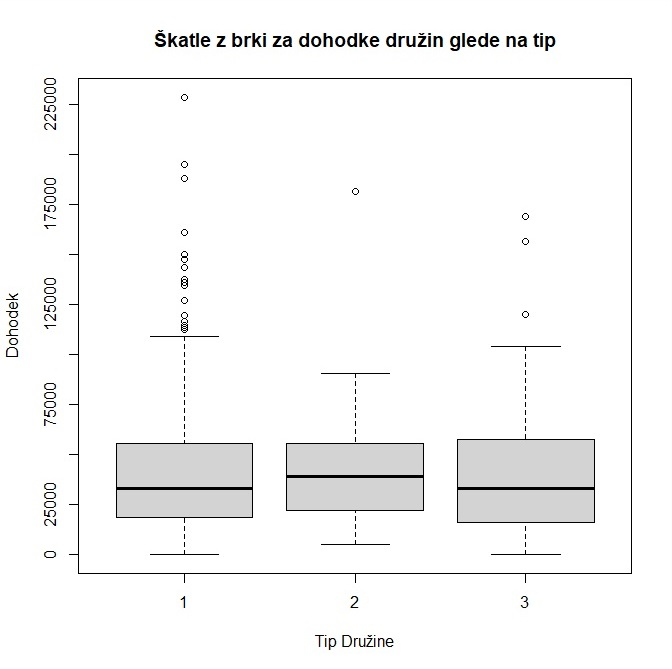
\includegraphics[scale = 0.5]{TabelaSample1}
	\caption{Vzporedno narisane škatle z brki tipov družin $1$, $2$ in $3$}
\end{figure}

Pri tem je vredno omeniti, da ordinatna os zavzema vrednosti med $-10000$ in $240000$ zaradi boljše vidljivosti robnih delov škatel z brki. Ker so razlike med maksimumi razmeroma majhne (Do te mere, da nas ne ovirajo preveč pri ogledu), lahko prikažemo kar cele škatle, brez da bi kakšen del skrajšali za boljšo razločnost. 

Škatle z brki nam sicer tudi ponudijo nekaj presenetljivih ugotovitev. V minimalnih dohodkih ni velikih odstopanj, razen pri tipu $2$, ki ima za razliko od ostalih pozitiven minimalen dohodek. Če ignoriramo ostale vzorce in tem rezultatom naivno verjamemo, so enostarševske družine z očetom (torej družine tipa $2$) z nizkim dohodkom relativno bolj premožne od ostalih tipov. To domnevo navidezno podpira tudi opazka, da je prvi kvartil pri tipu $2$ višji kot pri ostalih dveh tipih. Enako velja tudi za mediano. Šele pri tretjem kvartilu ostala dva tipa premagata drugi tip. Od tod lahko naivno sklepamo, da

\end{document}